\documentclass[,hyphens]{sigchi}

% Use this section to set the ACM copyright statement (e.g. for
% preprints).  Consult the conference website for the camera-ready
% copyright statement.

% Copyright
\CopyrightYear{2020}
%\setcopyright{acmcopyright}
\setcopyright{acmlicensed}
%\setcopyright{rightsretained}
%\setcopyright{usgov}
%\setcopyright{usgovmixed}
%\setcopyright{cagov}
%\setcopyright{cagovmixed}
% DOI
\doi{https://doi.org/10.1145/3313831.XXXXXXX}
% ISBN
\isbn{978-1-4503-6708-0/20/04}
%Conference
\conferenceinfo{CHI'20,}{April  25--30, 2020, Honolulu, HI, USA}
%Price
\acmPrice{\$15.00}

% Use this command to override the default ACM copyright statement
% (e.g. for preprints).  Consult the conference website for the
% camera-ready copyright statement.

%% HOW TO OVERRIDE THE DEFAULT COPYRIGHT STRIP --
%% Please note you need to make sure the copy for your specific
%% license is used here!
% \toappear{
% Permission to make digital or hard copies of all or part of this work
% for personal or classroom use is granted without fee provided that
% copies are not made or distributed for profit or commercial advantage
% and that copies bear this notice and the full citation on the first
% page. Copyrights for components of this work owned by others than ACM
% must be honored. Abstracting with credit is permitted. To copy
% otherwise, or republish, to post on servers or to redistribute to
% lists, requires prior specific permission and/or a fee. Request
% permissions from \href{mailto:Permissions@acm.org}{Permissions@acm.org}. \\
% \emph{CHI '16},  May 07--12, 2016, San Jose, CA, USA \\
% ACM xxx-x-xxxx-xxxx-x/xx/xx\ldots \$15.00 \\
% DOI: \url{http://dx.doi.org/xx.xxxx/xxxxxxx.xxxxxxx}
% }

% Arabic page numbers for submission.  Remove this line to eliminate
% page numbers for the camera ready copy
\pagenumbering{arabic}

% Load basic packages
\usepackage{balance}       % to better equalize the last page
\usepackage{graphics}      % for EPS, load graphicx instead 
\usepackage[T1]{fontenc}   % for umlauts and other diaeresis
\usepackage{txfonts}
\usepackage{mathptmx}
\usepackage[pdflang={en-US},pdftex]{hyperref}
\usepackage{color}
\usepackage{booktabs}
\usepackage{textcomp}

% Some optional stuff you might like/need.
\usepackage{microtype}        % Improved Tracking and Kerning
% \usepackage[all]{hypcap}    % Fixes bug in hyperref caption linking
\usepackage{ccicons}          % Cite your images correctly!
% \usepackage[utf8]{inputenc} % for a UTF8 editor only

% If you want to use todo notes, marginpars etc. during creation of
% your draft document, you have to enable the "chi_draft" option for
% the document class. To do this, change the very first line to:
% "\documentclass[chi_draft]{sigchi}". You can then place todo notes
% by using the "\todo{...}"  command. Make sure to disable the draft
% option again before submitting your final document.
\usepackage{todonotes}

% Paper metadata (use plain text, for PDF inclusion and later
% re-using, if desired).  Use \emtpyauthor when submitting for review
% so you remain anonymous.
\def\plaintitle{SIGCHI Conference Proceedings Format}
\def\plainauthor{First Author, Second Author, Third Author,
  Fourth Author, Fifth Author, Sixth Author}
\def\emptyauthor{}
\def\plainkeywords{Authors' choice; of terms; separated; by
  semicolons; include commas, within terms only; this section is required.}
\def\plaingeneralterms{Documentation, Standardization}

% llt: Define a global style for URLs, rather that the default one
\makeatletter
\def\url@leostyle{%
  \@ifundefined{selectfont}{
    \def\UrlFont{\sf}
  }{
    \def\UrlFont{\small\bf\ttfamily}
  }}
\makeatother
\urlstyle{leo}

% To make various LaTeX processors do the right thing with page size.
\def\pprw{8.5in}
\def\pprh{11in}
\special{papersize=\pprw,\pprh}
\setlength{\paperwidth}{\pprw}
\setlength{\paperheight}{\pprh}
\setlength{\pdfpagewidth}{\pprw}
\setlength{\pdfpageheight}{\pprh}

% Make sure hyperref comes last of your loaded packages, to give it a
% fighting chance of not being over-written, since its job is to
% redefine many LaTeX commands.
\definecolor{linkColor}{RGB}{6,125,233}
\hypersetup{%
  pdftitle={\plaintitle},
% Use \plainauthor for final version.
%  pdfauthor={\plainauthor},
  pdfauthor={\emptyauthor},
  pdfkeywords={\plainkeywords},
  pdfdisplaydoctitle=true, % For Accessibility
  bookmarksnumbered,
  pdfstartview={FitH},
  colorlinks,
  citecolor=black,
  filecolor=black,
  linkcolor=black,
  urlcolor=linkColor,
  breaklinks=true,
  hypertexnames=false
}

% create a shortcut to typeset table headings
% \newcommand\tabhead[1]{\small\textbf{#1}}

% End of preamble. Here it comes the document.
\begin{document}

\title{We are the Greatest Showmen: Configuring Mobile Learning Technologies for Student-Led Activities}

\numberofauthors{3}
\author{%
  \alignauthor{Leave Authors Anonymous\\
    \affaddr{for Submission}\\
    \affaddr{City, Country}\\
    \email{e-mail address}}\\
  \alignauthor{Leave Authors Anonymous\\
    \affaddr{for Submission}\\
    \affaddr{City, Country}\\
    \email{e-mail address}}\\
  \alignauthor{Leave Authors Anonymous\\
    \affaddr{for Submission}\\
    \affaddr{City, Country}\\
    \email{e-mail address}}\\
}

\maketitle

\begin{abstract}
While the use of mobile learning technologies by teachers and community experts has been explored by HCI research, little attention has been given to how they could enhance learning activities designed by the students themselves. Following an action research approach, we report on engagements inside and outside of the classroom with both teachers and students from three different UK schools, using a variety of configurations to work within given time constraints and produce student-led mobile learning activities using the OurPlace application. We also report on the use of the OurPlace to facilitate an exchange of knowledge and values between a class from an ethnically diverse inner-city school and the children of a community of travelling Showmen. We contribute insights gained from these studies, and offer suggestions for how project-based mobile learning technologies can be better configured within the restrictions of a formal education environment to support student independence, heritage learning and the exchanging of values.
\end{abstract}


% ACM Classfication

\begin{CCSXML}
<ccs2012>
<concept>
<concept_id>10003120.10003121</concept_id>
<concept_desc>Human-centered computing~Human computer interaction (HCI)</concept_desc>
<concept_significance>500</concept_significance>
</concept>
<concept>
<concept_id>10003120.10003121.10003125.10011752</concept_id>
<concept_desc>Human-centered computing~Haptic devices</concept_desc>
<concept_significance>300</concept_significance>
</concept>
<concept>
<concept_id>10003120.10003121.10003122.10003334</concept_id>
<concept_desc>Human-centered computing~User studies</concept_desc>
<concept_significance>100</concept_significance>
</concept>
</ccs2012>
\end{CCSXML}

\ccsdesc[500]{Human-centered computing~Human computer interaction (HCI)}
\ccsdesc[300]{Human-centered computing~Haptic devices}
\ccsdesc[100]{Human-centered computing~User studies}

% Author Keywords
\keywords{\plainkeywords}

% Print the classification codes
\printccsdesc
Please use the 2012 Classifiers and see this link to embed them in the text: \url{https://dl.acm.org/ccs/ccs_flat.cfm}



\section{Introduction}

Introduce context school pressures, limitations
Rising role of mobile technology

\section{Related Work}

\subsection{Constructionism}
The learning theory of constructionism, introduced by Seymour Papert in the mid-1980s, argues that constructing, sharing and reflecting upon physical or virtual `public entities' can be a powerful way for learners to build `knowledge structures'--collections of knowledge, concepts and facts interrelated through various semantic relationships \cite{PapertSeymourandHarel1991a}. Papert argues that the process of learning is the building of these knowledge structures, a process which--while it occurs irrespective of the circumstances of the learning--happens `\textit{especially felicitously in a context where the learner is consciously engaged in constructing a public entity}'. These public entities could range from physical artefacts such as models of buildings, virtual programming code or even conceptual theories of the universe. In their overview of constructionism, Noss and Hoyles use Logo (a simple programming environment which included a `turtle' entity, whose movements around the screen could be programmed \cite{Harvey1997}) as an example of a constructionist working environment \cite{Noss2017}. They argue that this environment offered a medium in which learners could `\textit{explore and learn from feedback, much as one can master a foreign language by living in the appropriate country}'. Noss and Hoyles also claim that Logo's environment affords learners to take ownership of a construction-based approach, potentially leading to greater engagement, confidence and empowerment. Finally, they posit that through exploration and construction of public entities, learners can encounter `powerful ideas': `\textit{concepts and strategies  that confront and build upon intuitive knowledge}'. For this reason, Noss and Hoyles argue that constructionist tools need to be expressive enough to facilitate these ideas emerging through the learner's construction of public entities.

\subsection{Project-Based Learning}
Blumenfeld et al note that small, easily assessed tasks which focus on low-level facts and skills (e.g. tasks commonly found on worksheets) have become the focus of American classrooms \cite{Blumenfeld1991}. However, they argue that these tasks afford students `\textit{few opportunities to represent knowledge in a variety of ways, pose and solve real problems, or use their knowledge to create artifacts}'. They argue that a preferable alternative is project-based learning (PBL), which they describe as an approach to teaching and learning which focuses on engaging students through the investigation of non-trivial, `authentic' problems in a manner which supports learner autonomy over the course of an extended project. Frequently, these projects will result in the creation of an artifact in response to a given question or problem (such as videos, reports, artworks, websites or performances \cite{Holubova2008}), in effect making PBL a method of applying constructionism in response to real-world problems and supporting the inclusion of prior knowledge, domain research and greater levels of student autonomy. It's worth noting that several other configurations of PBL have been developed over time (e.g. problem-based learning), however they mostly conform to the same essential elements: a challenging problem or question; sustained inquiry; an element of authenticity; a degree of student control; reflection; critique and revision; and a final public product \cite{Larmer2015}. Previous research has argued that these projects can serve to build bridges between classroom activities and real-life experiences \cite{Blumenfeld1991}, enhance applied and conceptual knowledge around a subject \cite{Boaler1999}, and that PBL's greater levels of autonomy and challenge can result in higher levels of student engagement \cite{Wurdinger2007}.

Project-based learning is also recognised as fertile ground for technology-enhanced learning. Bell argues that `\textit{technology as a means, not an end, enables students to experiment with different technologies for all aspects of PBL}' (including research and data collection, knowledge sharing and artifact creation) and that it can be `\textit{highly engaging to students, because it taps into their fluency with computers}' \cite{Bell2010}. ChanLin describes how students used digital technologies within PBL for researching on the web, taking photographs, participating in online communities and creating web pages as final artifacts \cite{ChanLin2008}. Krajcik et al note that while the use of mobile and desktop technologies help students build knowledge structures and form deeper and richer understandings of the subjects at hand, teachers frequently run into challenges in gaining access to computing hardware due to multiple classes sharing resources \cite{Krajcik2006}.

While some studies have found that project-based instruction is not necessarily more demanding in terms of teaching time and resources \cite{Al-Balushi2014}, Blumenfeld et al posit that by its nature PBL `\textit{requires active engagement of students' effort over an extended period of time}' \cite{Blumenfeld1991}. Krajcik et al argue that `\textit{it takes more time to complete a task where students are constructing their own knowledge in meaningful, situated activities}', leading to teachers being hesitant to put it into practice when faced with strict and competing curriculum goals \cite{Krajcik2006}. The non-profit organisation Innovation Unit note `\textit{[PBL] can be a powerful learning strategy if it is part of a whole school change process, and [schools] are ready and able to make the necessary time and staff available}' \cite{InnovationUnit2016}, suggesting that putting PBL into practice requires substantial changes in how teachers approach classroom structures, activities and tasks. This is easier said than done, particularly when teachers and schools work within structures which pressure them to conform to quantifiable testing methods, propagating the aforementioned worksheet-style tasks and `teaching to the test'. For example, the head of the UK's Office for Standards in Education (Ofsted) has noted that `\textit{[Ofsted] have created a situation where second-guessing the test can trump the pursuit of real, deep knowledge and understanding}' \cite{Ofsted2018}. All of these factors result in varying levels of restrictions placed upon teachers, impacting their time affordances, curriculum content and pedagogical approaches. This has meant that  implementing project-based learning in UK schools has proven to be a challenge \cite{TheEducationEndowmentFoundation2016}.

\subsection{The TPACK Framework}

The Technological Pedagogical Content Knowledge framework (TPACK) provides a model which describes the roles of and interactions between what Koehler and Mishra argue are the three main components of teachers' knowledge: content, pedagogy and technology \cite{Harris2009}. In the model, content knowledge refers to the teacher's knowledge about the domain and subject matter to be learned or taught; technological knowledge refers to an evolving understanding of how technology could assist or impede the achievement of a goal; and pedagogical knowledge is the teacher's understanding of the processes, practices and methods of teaching and learning. Furthermore, each of these interact with each other (for example, technological pedagogical knowledge describes an understanding of how teaching and learning can change when technologies are used in different ways), and exist within diverse contexts (e.g. environmental, socioeconomic). 

Koehler and Mishra argue that when taken as a whole, the TPACK framework describes `\textit{the basis for effective teaching with technology}', including how technologies can be used effectively within the teaching process for representing new concepts and building upon existing student knowledge. They also posit that any changes in one of the three main components has to be `compensated' by changes to the other two. They note that this is frequently seen with technology, as it can be rapidly evolving, opaque in its inner-workings and multi-purpose. One given example is the increasing usage of the Internet for online learning, which forced educators to think about how educational content can be represented in new ways on the web, and how it can be used to connect students to content, communities and each other.  The authors argue that the model discourages teachers and researchers from `\textit{oversimplified approaches which treat technology as an add-on'}, and instead regarding teachers' technology knowledge as being in a dynamic equilibrium with content and pedagogical knowledge.

\subsection{Mobile Learning}

Mobile learning (`\textit{learning across multiple contexts, through social and content interactions using personal electronic devices}' \cite{Crompton2013}, AKA `m-learning') has continued to play a large role within schools in the UK, with ready access to tablet computers becoming more common in schools (44\% of UK schools are expected to have one tablet per child by 2020 \cite{BritishEducationalSuppliersAssociation2015}), and their general ubiquity meaning most of the younger population is familiar with their use (87\% of UK adults report owning a smartphone \cite{Statistica2018}, as do 84\% of children aged between 8-16 \cite{Statistica2018a}). While traditional desktop and laptop devices are currently still more common in schools (numbering approximately 3.4 million in 2017 \cite{BritishEducationalSuppliersAssociation2017}), mobile devices have been touted as having a number of advantages over their more stationary counterparts: for example, Traxler argues that mobile technologies can offer structured educational experiences which can be situated in--and responsive to--authentic learning environments \cite{Traxler2011}. This makes m-learning a potentially great fit for subscribers to Lave and Wenger's Situated Learning Theory, which posits that learning unintentionally occurs in authentic activities, contexts and cultures through `legitimate participation' in communities of practice \cite{Lave1991}. Sharples et al argue that to better utilise these advantages, m-learning technologies should take into account the physical and social aspects of the learning context (both physical and social); the amount of control the learner has over the activity; and the learner's communication with others \cite{Sharples2007}.

Previous m-learning research has used these capabilities for a wide variety of applications, such as sensing tool kits to conduct citizen science \cite{Sharples2017}; enabling seamless learning across classrooms and museums on school trips \cite{Vavoula2009}; and empowering children in collecting evidence to support their advocacy and engagement in urban design processes \cite{Peacock2018}. Prior research has also shown that m-learning technologies can enhance the development of relationships with place, and act as a medium through which stakeholders can harness the underlying socioeconomic infrastructures of place as learning resources \cite{Richardson2017}. In the ParkLearn project, Richardson et al attempted to combine elements of all of the above into a single mobile application supporting creating, sharing and engaging with bespoke, place-based m-learning activities `\textit{that leverage the targeted learning environment and mobile devices' hardware to support situated learning}' \cite{Richardson2018}. Through using ParkLearn in longitudinal studies with a primary school and volunteers at a local park, the authors found that the app promoted a sense of ownership in both learners and activity creators by supporting greater degrees of creativity and independence. Furthermore, the app was shown to be an effective medium through which physical and social aspects of the local environment could be leveraged as learning resources.

Chan et al note that the use of mobile technologies in PBL has been under-researched \cite{Chan2015}. In a qualitative study with an undergraduate course, they noted that students used mobile devices for multiple stages of the PBL process, including researching the subject on the Internet, making notes, sharing materials and making use of educational applications to help understand abstract concepts. Massey et al took a different approach, presenting graduate-level students with the challenge of creating a mobile-friendly version of their course-management software, with the created software acting as the final public entity of the students' team projects \cite{Massey2006}. They argue that this pedagogical environment aimed to re-frame the students as `\textit{not only end users of mobile applications, but also as developers and decision makers}'. These studies suggest that like other forms of classroom technology, m-learning technologies can be configured to support the PBL process, or even be used to construct the project's final public entity.

\section{A Project Based Mobile Learning Curriculum}

With these studies in mind, we decided to explore how project based m-learning  (PBML) could be effectively configured within the context of UK schools. In order to capitalise on the advantages of mobile learning technologies, we decided that any educational projects should take a situated learning approach which leveraged the schools' surrounding heritage as educational resources. As the ParkLearn application's activities were reported as being well suited to this, we believed that the construction of an activity regarding local heritage would be a good final public entity for a project. In this section we introduce the latest iteration of ParkLearn, OurPlace, and the short curriculum we created to use it as a PBML tool within UK schools.

\subsection{The OurPlace App}

OurPlace is the current iteration of the open-source ParkLearn platform, with an expanded feature set and re-branded to support its use in contexts outside of local parks \cite{Richardson2018a}. Consisting of a website and mobile applications for both Android and iOS, OurPlace supports the creation of--and sharing and engagement with--m-learning activities (`Activities'), each of which is built up from smaller, modular tasks (`Tasks'). These tasks each consist of a specific interaction (`Task Type'), which either promote creativity, emulate traditional classroom learning materials or use the device's hardware to give context-specific experiences (Table~\ref{tab:TaskTypes}). With the exception of \textit{Scan the QR Code}, all of these Task Types were present in the original ParkLearn application. An Activity can have any number of Tasks within it. OurPlace also adds support for `Follow-Up Tasks', which allow activity creators to add sub-tasks which unlock once their parent task has been completed (Figure~\ref{fig:ActivityCreation}.e). This supports the design of more complicated combinations of interactions (for example: a \textit{Location Hunt} could unlock a \textit{Record Audio} and \textit{Take a Photo} once the user arrives at a designated location, or a \textit{Multiple Choice} could quiz the user about what they've just heard in a \textit{Listen to Audio}).

\begin{table}
  \centering
  \begin{tabular}{l|p{50mm}}
    % \toprule
    {\small\textit{Task Type}}
    & {\small \textit{Interaction Description}} \\
    \midrule
    Information & Read some written information, with an optional accompanying image and hyperlink to a web page \\
    Listen to Audio & Listen to a given audio recording \\
    Take a Photo & Use the camera to take still images in response to an instruction \\
    Photo Match & Use the camera to match an existing photo given as an overlay \\
    Draw a Picture & Draw a picture onto a blank canvas \\
    Draw on Photo & Draw on top of a given image \\
    Record Video & Record a video using the camera \\
    Record Audio & Record an audio clip using the device's microphone \\
    Map Marking & Mark a given number of locations onto a Google Map \\
    Location Hunt & Track down a target location by observing your reported distance from it \\
    Scan the QR Code & Find and scan the correct QR code \\
    Multiple Choice & Choose a response from a set of text options \\
    Text Entry & Enter a response using the device's keyboard
    % \bottomrule
  \end{tabular}
  \caption{The Task Types available in the OurPlace application}~\label{tab:TaskTypes}
\end{table}

\begin{figure*}
  \centering
  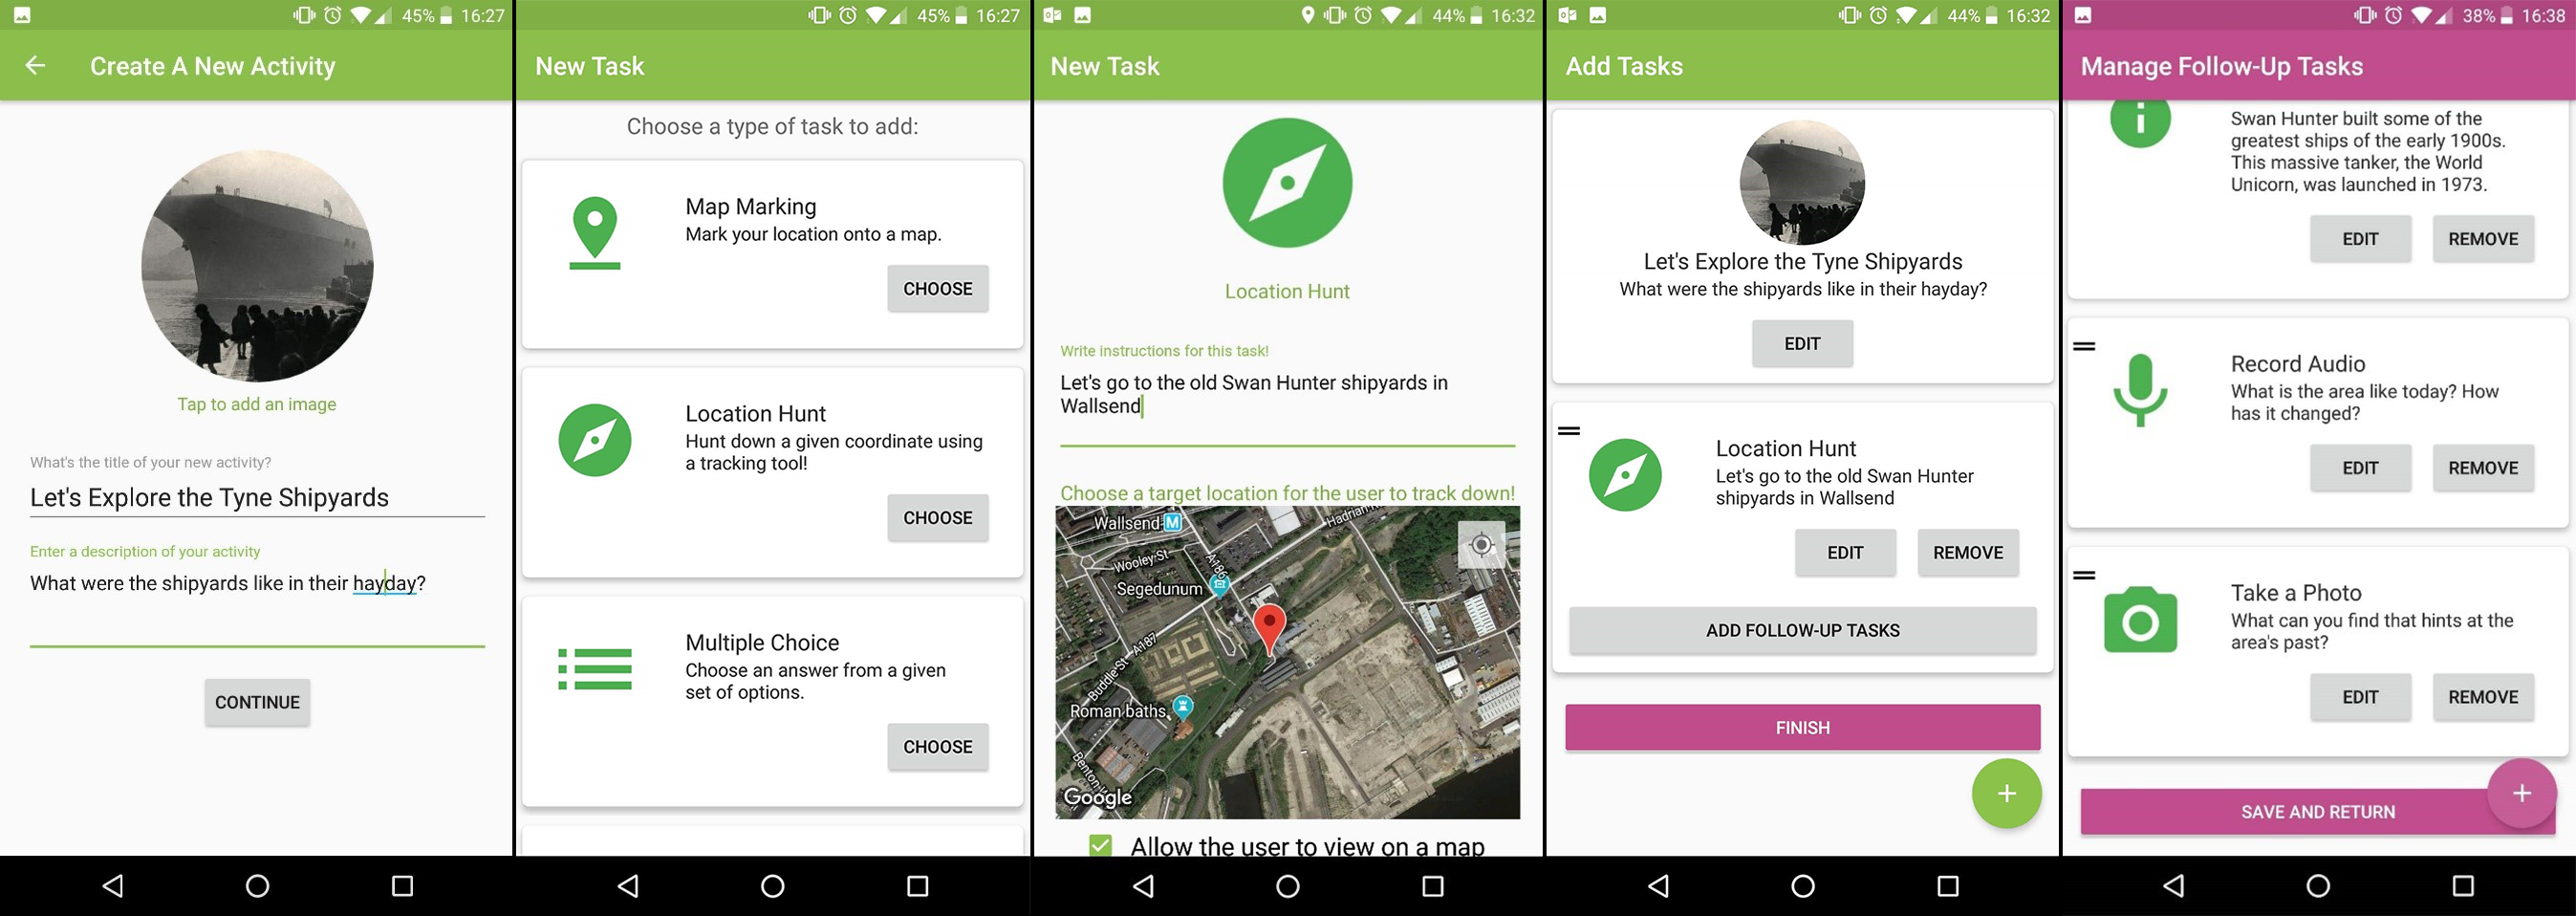
\includegraphics[width=2.1\columnwidth]{figures/activityCreation}
  \caption{Creating an OurPlace activity (left to right): a) Choosing the activity's title, description and image; b) Choosing a Task Type to add; c) Adding a \textit{Location Hunt} Task, with description and target coordinates; d) The new Task in the Activity; e) Adding Follow-Up Tasks to the \textit{Location Hunt}  }~\label{fig:ActivityCreation}
\end{figure*}

Activities are created within the app itself. After supplying a title, description and an optional image (Figure~\ref{fig:ActivityCreation}.a), the designer creates the Tasks that make up the Activity (Figure~\ref{fig:ActivityCreation}.b). Each Task Type requires at least a written instruction for the learner (e.g. A \textit{Location Hunt} might say \textit{`Can you find Carter's Well?'}), but some of them require some additional customization (e.g. supplying geographic coordinates by tapping on a Google Maps view) (Figure~\ref{fig:ActivityCreation}.c). When a Task Type requires an additional file (e.g. a target image for \textit{Photo Match} or an audio recording for \textit{Listen to Audio}), creators are able to either create them through the app itself or load it from an external source (such as Google Drive, Dropbox or files otherwise downloaded from the web). This means that no additional equipment or software is required to create activities (other than \textit{Scan the QR Code}, which requires creators to print the generated QR code from the OurPlace website). Once finished, Activities can be tagged as being relevant to a location before uploading, making it easier for others to find. Additionally, QR codes which launch the activity when scanned in the app can be printed from the OurPlace website. Uploaded activities can be edited for testing, feedback and iteration--allowing for the `essential elements' of reflection, critique and revision of a final public product \cite{Larmer2015}. 


\subsection{Overview of the OurPlace Curriculum (IRPAPE)}

From previously identified issues encountered by past researchers and practitioners when implementing project based learning projects in schools \cite{Blumenfeld1991, Krajcik2006, InnovationUnit2016, TheEducationEndowmentFoundation2016}, we knew that any programme of activities would have to be able to adapt to variations in teachers' time and levels of mobile hardware access. In response, we designed an adaptable six-stage curriculum, which could span from dozens of hours of teaching time to only a handful (through omission of stages). This curriculum asks students (either individually or in groups) to create an OurPlace Activity as a final public entity, following a series of PBL engagements in response to their teacher's chosen topic. The stages--and the reasoning behind them--are described below. These have been designed with the OurPlace application in mind, however we believe the curriculum could be adapted to other learning technologies.

\subsubsection{Introducing the Medium (I)}
This first stage involves the students becoming familiar with the OurPlace application: its feature set, the structure of an Activity (including the potential for Follow-Up Tasks) and some examples of how the different Task Types can be implemented. This would ideally be performed on the school grounds with an example Activity, created to demonstrate all of the different Task Types available to the students. Doing this on the school grounds allows students to explore the application in a safe outdoor environment, and doesn't require the overhead of additional teaching assistants (more adults are often required when leaving the school grounds). Doing this first will allow students to bear the capabilities of the technology in mind and help them formulate ideas during the following stages.

\subsubsection{Researching the Domain (R)}
As with most other forms of PBL, a significant amount of time is allotted to students investigating the given problem domain. This is likely to be assisted in some way by technology, however other options exist such as fieldwork (e.g. site visits, performing interviews) and offline research (e.g. in libraries). A degree of autonomy should be granted to the students, however some guidance may be required (pointing them towards good resources, for example).

\subsubsection{Prototyping (P)}
In this stage, students create a low fidelity, pen and paper prototype of their Activity using their research as content. For this series of studies we created a `jigsaw' exercise, where students can design and play with different configurations of their OurPlace Activities without having to simultaneously learn the app's authoring interface (Figure~\ref{fig:Jigsaw}). It also means that the students can start designing their Activities without access to mobile hardware. The jigsaw's structure is directly analogous to that of an OurPlace Activity: a single piece is dedicated to the Activity's title, description and cover image (i.e. Figure~\ref{fig:ActivityCreation}.a), with the Activity's Tasks represented as separate pieces connecting to it and chaining together. Each Task's jigsaw piece has a slot for a Task Type, and the jigsaw's connectors allow for pieces to be connected in different directions (e.g. to indicate Follow-Up Tasks). Pieces were given a layer of sticky-back plastic and written on with dry-wipe pens, allowing  both the students to make amendments and the jigsaws to be reused. Once students were happy with their final jigsaw configuration, the prototypes were photographed for later reference. The jigsaw design is included in the supplementary materials.

\begin{figure}
\centering
  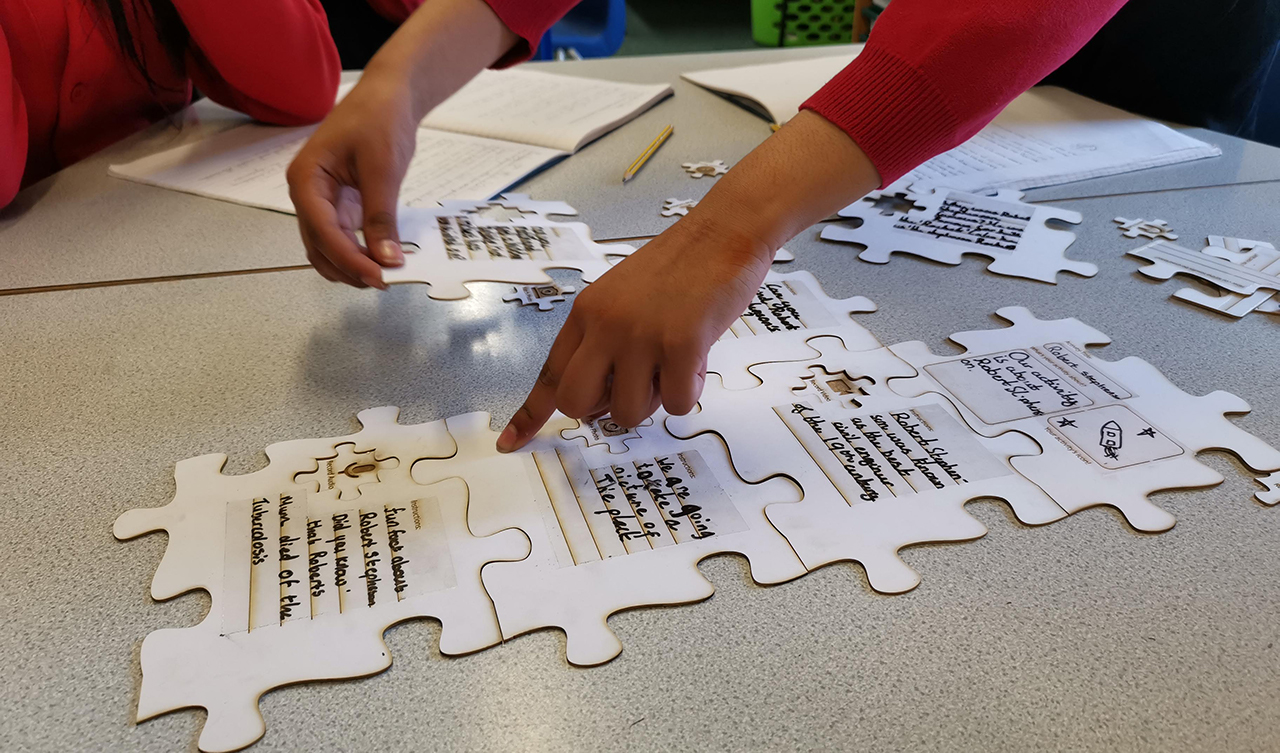
\includegraphics[width=1\columnwidth]{figures/jigsaw}
  \caption{The jigsaw exercise, in which students created pen and paper prototypes of OurPlace Activities using their research notes.}~\label{fig:Jigsaw}
\end{figure}

\subsubsection{Assembling \& Refining (A)}

This stage involved the creation of the Activity within the OurPlace app itself, and requires some instruction from the educator/researcher as to how the app's creation process works. If the students created a prototype, this simply serves as a digitisation process. Once finished and uploaded, students may want to try their Activities (location allowing) and refine them in response to any issues they encounter.  

\subsubsection{Sharing with Peers in the Wild (P)}

With the final versions uploaded, students exchange Activities with each other and run them in the authentic learning environment. Ideally, this would also include an element of peer feedback afterwards.

\subsubsection{Sharing Externally in the Wild (E)}

The final stage takes the students' Activities and frames them as literal public entities, accessible within the authentic learning context for communities outside of the school to be able to access.

\section{Studies}

We wanted to assess how well this curriculum would work when applied within a real school context and--given the time and resource limitations frequently found within schools--how it could be configured to adapt to a given school's constraints. In this section we discuss studies held with three different formal education schools in the North East of England, as well as engagements held with a summer school of Travelling Showmen. Each has their own socio-economic and cultural backgrounds and unique locality. As a point of comparison, we also include a brief discussion of a planning meeting with teachers from a fourth school. For easy reference, we've created a notation showing which elements of the IRPAPE curriculum were present in each study, replacing any omitted stages with dashes.

\subsection{Research Methods \& Data Collection}

Unless noted otherwise, all student interactions with the OurPlace application took place through Android tablets provided by the researchers, with the tablets' Internet connectivity provided by the researchers' wireless router and SIM card. The first author was present whenever the app was in use (unless noted), providing technical support as necessary and taking field notes and audio recordings. No identifiable information on the student participants was collected with the exception of photographs, which were only taken with prior parental consent. Any names given below are pseudonyms. Semi-structured interviews were held with the teachers after the engagements, with a mixture of oral and written feedback given by students. A thematic approach to coding was performed across all of this data, with codes being qualitatively analysed by the authors before grouped into final agreed-upon themes.

\subsection{Study 1: Extreme Time-Limitations (IR-A-\--)}
The first group we engaged with was a Year 8 history class (age 12-13, N=32) in a secondary school (School 1) based in a moderately affluent village. We approached the school's leadership about the possibility of them using the app: the school's headteacher agreed and assigned the class's history teacher (Teacher 1) to the study. School 1 appeared to have a very `traditional' teaching environment--as with many other secondary school teachers in the UK, Teacher 1 was under pressure to prepare the students for frequent formal assessments, and so was reluctant to dedicate much teaching time to the project. When we were organising the study, he noted: `\textit{Workload and time would be the main issues--the commitment it would take up in lesson time. It would be difficult to slot something additional like this in around key assessment work, and also keeping it relevant to the curriculum we are following}'. As a result, the project was given a very short amount of classroom time--only two hour-long sessions, with further work to be done by students outside of school. Observations of two of Teacher 1's other lessons suggested that he preferred an `authority' or lecture style of teaching: lessons were teacher-centred, with students expected to take notes on content that was delivered to them and answer occasional questions raised by the teacher. Teacher 1 appeared ambivalent towards PBL approaches, and when queried on his opinion of them simply noted `\textit{It's not the way we do things here}'.

Teacher 1 already possessed a paper-based history trail of the local village, designed for use by new, younger students joining the school. For the study, Teacher 1 tasked his class to use OurPlace to create a digital trail, featuring historical elements of their choosing. Prior to our first session with the students, he provided them with a comprehensive and lengthy PDF document, which detailed most--if not all--of the historical buildings in the village, serving a starting point for researching content. He also provided the students with the existing trail and a PowerPoint presentation containing information pulled and summarised from the PDF. As a result, prior to the first session, Teacher 1 expected that the students should be fairly well prepared in terms of trail content: `\textit{The students should already have ideas of what they want to do, but are waiting to see what the software will do. The issue is what the software can do and whether it can easily tied in with the plans they have made already.}'  As such, the \textit{Researching the Domain} stage was present, albeit earlier in the process than we had anticipated. 

Teacher 1 was also concerned about the students' work being able to work outside of a mobile learning context, hoping to also have `analogue' versions of the students' trails: `\textit{Ideally, what is done needs to be able to be adapted to be used again. The bespoke software side of it does worry me a bit in this regard. Could a finished product be adapted to be used at another time even if no iPads were available--maybe some of the ideas usable in a non-digital way?}'. To this end, he encouraged students to try and design their digital trails such that they would be adaptable to a pen and paper format.

Teacher 1 decided to make the majority of the Activity creation process a homework task, with students using their own smart devices outside of school. This was mainly in response to the extremely limited amount of classroom teaching time that could be dedicated to the project: because we also wanted to go through the students' final Activities with them, that only left a single hour-long session to work with the students in class. In order to prepare the students for this independent work, our first hour-long session was spent \textit{Introducing the Medium}. This involved the students completing an example OurPlace Activity on the school grounds, demonstrating all of the Task Types and several instances of Follow-Up Tasks. Upon return to the classroom, the rest of the session (around 20 minutes) was spent introducing the students to the Activity creation tools in the app. By the end of the hour, all students reported that they understood the app, what it could do and how to make their own Activity.

We returned to the school three weeks later for the second session, in which the first author and Teacher 1 sat with the students and went through their Activities with them. While most of the students had produced an Activity, they tended to be quite short (averaging X Tasks per Activity) and shallow: most of the Activities served more as explorations of the different interactions possible with the app than a meaningful engagement with the subject matter. For example, one student's Activity asked the learner to simply find and photograph an `area of interest', putting greater focus on the technology than the learning content. As a result, many students struggled in fulfilling the teacher's requirement of creating a paper-based version of their Activity. However, one pair of students had more success, claiming `\textit{I think we've found it easier than other groups because we focused more on the content than using all of the different interactions. So a lot of the content can be the same, it's just changing how to interact with it}'. 

When giving feedback to the class, Teacher 1 also pointed out that even where their Activities might contain some meaningful content, they aren't necessarily good for learning from: `\textit{What needs some further thought is what you're actually asking them to do in terms of the content. What are they doing in order to get that information? They can't pluck things out of thin air if they have no idea. Feed them some information, then wherever they are at they can work out the rest.}' He then offered some ideas of how the features of the technology could be used as a teaching tool: `\textit{Or send them specifically to somewhere where they can work out the answer to something. Use of old images in this technology I think might work. You know, send them to a place with an old photograph. Get them to do some comparisons, get them to think about why things have changed}'.

Teacher 1 had also noticed the students' focus on interactions with the technology over engaging more deeply with the historical content. In the follow-up interview, he noted: `\textit{I don't know about you but the thing I was coming across again and again was the lack of challenge, the lack of depth, and the kind of things they were asking was really just playing with the technology rather than [engaging with the history]}'. This surprised him, as he had been expecting any issues encountered to have resulted from the introduction of new technology, rather than the students' research--especially as they had been given the resources so early on: `\textit{I think it's more of a success for the technology, the medium, than the actual content. [...] Maybe not what I expected, actually--in some ways maybe the opposite}'. He argued that without the deeper integration of research and knowledge into the Activities, they are of little value: `\textit{It needs to be worth doing: there's no point in having all of the bells and whistles if there's no substance}'. He noted that this could have been improved through a reconfiguration of the engagements, suggesting that more structured, scaffolded activities could have guided the students to produce more successful projects: `\textit{It's worth cogitating about what parameters you probably need to introduce, to guide them towards deeper thinking. I know that if that had been more free-form and open-ended, that would have been rather worse}.' He suggested that when applying content knowledge to Activities, a balance needed to be struck between a more guided, restrictive approach and supporting students' creativity and autonomy: `\textit{If they were highly creative and lost their focus, then they'd be miles [off]. If they were less creative, but focused on the nature of the content, they'd probably find it easier to transpose. What we want is something in-between}'.

\subsection{Study 2: Without Sharing Externally (IRPAP-)}
We worked with two different schools over an extended period of time (10-12 hours of sessions per school, spread over several weeks) to deliver a more fully-implemented version of the curriculum. This was partly supported by the fact that we were working with Year 4 (age 8-9) classes in both schools--as less focus is placed on preparing for examinations at these early ages, we've found (anecdotally, through previous research engagements) that pre-secondary school teachers are more willing to engage with experiential and exploratory forms of learning, rather than simply `teaching to the test'. As such, both schools welcomed the implementation of a longer project spread over several sessions.

The first of these schools (School 2) was based in a tiny rural village, and--due to the small population--we worked with the entirety of the Year 4 group, who were the oldest children in the school (age 8-9, N=7). Because each the school's population is so small, the school's classes are actually made up of several year groups--meaning that Year 4 and Year 3 share the same classroom. The class teacher (Teacher 2) had approached us about using the OurPlace app as a way to augment orientation and map-reading with new technologies in lessons. With this generous scope and large amounts of time available, we decided that the students would do two projects: one to learn the mechanics of making Activities in the app, and another which focused on local heritage in the village. 

For the first project, we tasked the Year 4 students with creating OurPlace Activities for their younger classmates to complete, with the only stipulation being that the Activities should be based around the school grounds. A Teaching Assistant was present throughout this first project, to help the lead researcher with any children who struggled. As with School 1, in the first two-hour session we \textit{Introduced the Medium} through an example Activity which demonstrated the app's capabilities. We then moved straight to the \textit{Prototyping} phase, as these first projects didn't require any research. While the students initially struggled conceptually with the jigsaws due to their abstract nature, after a few minutes they understood the links between the puzzle pieces and the structure of the app. We soon found that while students were generally favouring the Task Types which they found most interesting during the demo Activity--namely \textit{Take a Photo, Location Hunt} and \textit{Record Audio}--their Activities made use of most of the different Task Types available. We believe that this may have been encouraged by the jigsaw packs having a limited number of each Task Type piece, meaning that students were unable to make an Activity with many of the same Task Type (however, some students overcame this by simply not placing a Task Type piece if the right one wasn't available--see Figure~\ref{fig:JigsawToApp} as an example). The largest hurdle was around students' ideation of what the Activities should be about--with such a broad scope and without a subject focus, they struggled to think of different themes. They all settled on some form of `adventure', where each Task was a puzzle or riddle to solve in order to find locations within the school. The students' jigsaws were photographed at the end of the session.

\begin{figure}
\centering
  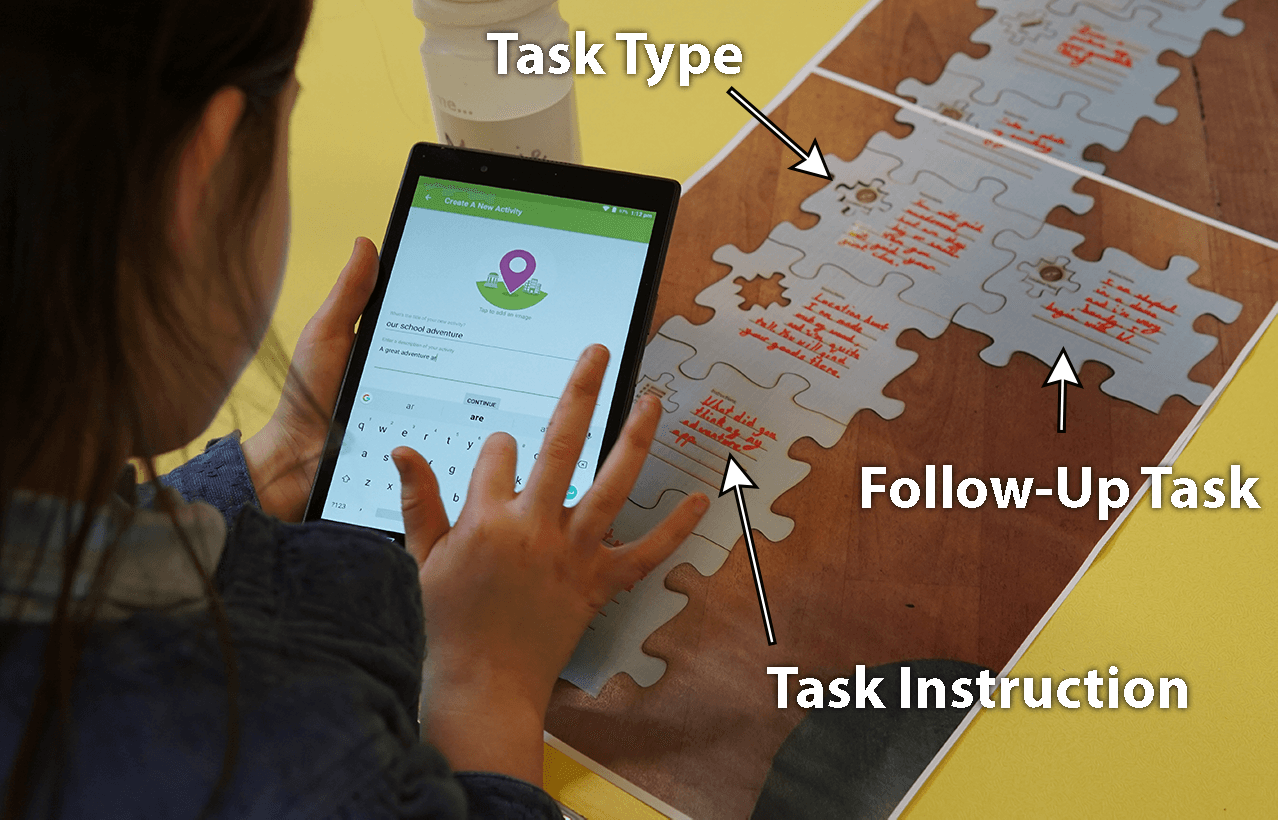
\includegraphics[width=1\columnwidth]{figures/jigsawToApp}
  \caption{A student uses a photograph of her jigsaw prototype as a reference for creating an OurPlace Activity.}~\label{fig:JigsawToApp}
\end{figure}

In the second two-hour session, during which the students \textit{Assembled} their OurPlace Activities, the photos were given to the students as references   (Figure~\ref{fig:JigsawToApp}). One of the students particularly struggled with typing with the on-screen keyboard, which Teacher 2 attributed to due to lower literacy skills. However, the others were happy working independently, and reported that their jigsaws made learning the creation process `\textit{much easier}'. The students had fun exploring what they could do with the app's functionality: for example, one student's final \textit{Listen to Audio} Task `rewarded' the user for completing his Activity with a recording of him singing \textit{Celebration} by Kool \& the Gang. The second session concluded with the students testing out their Activities and making a few refinements (mostly involving spelling errors and re-ordering Tasks). 

The final two-hour session of the project was spent by the students \textit{sharing with their peers}. Teacher 2 briefed the younger students, giving the Year 4s positions of seniority and highlighting their efforts: `\textit{You really need to listen to what [Year 4] have to say, because they have designed this themselves. They are your teacher, OK? Please listen, because they've worked really hard, and they're really excited about you having a go.}' The Year 4s accompanied rotations of small groups of younger students as they completed their Activities around the school, with groups being swapped to allow all students to try each Activity (the younger students were keen on making sure they completed all of them). The Year 4s were given the responsibility of showing the younger students how the app worked, and assisting them if they got stuck (Figure~\ref{fig:Mushrooms}). At the end of the session the Year 4s hosted a school assembly, in which they showed the other children their jigsaws and shared what they most enjoyed (`\textit{I enjoyed being the teacher'; `Being outside'; `I enjoyed making the Activity itself}') and the younger children gave feedback (\textit{`Our favourite was [Susan's], because we got to find lots of things'; `I really liked the beeping one, the Location Hunt'}). The school's headteacher praised the Year 4s' independent work as showing maturity: `\textit{We can trust you to do something away from the class teacher and still do something really good. I think you really are stepping up to be Year 4s, it's wonderful to see. [...] If you're very grown up, you get to do very grown up things. So let's give year 4 a clap}'. Teacher 2 also praised their leadership (`\textit{I would like to also point out how good they were as teachers, as well. They really came into their own. I was very proud of them.}') and noted that the OurPlace app supported a varied output: `\textit{They were very different as well weren't they? The ideas. Even though you all started off with the same tools'}. Finally, the headteacher noted that the Teaching Assistant had also been strongly engaged with the process: `\textit{Gabrielle said she was going to stay extra time, because she wanted to see how it was going to finish up. She worked overtime so she could see how [Year 4 were] getting on. So she was really interested as well}'.

Following the success of the first project, 

\begin{figure}
\centering
  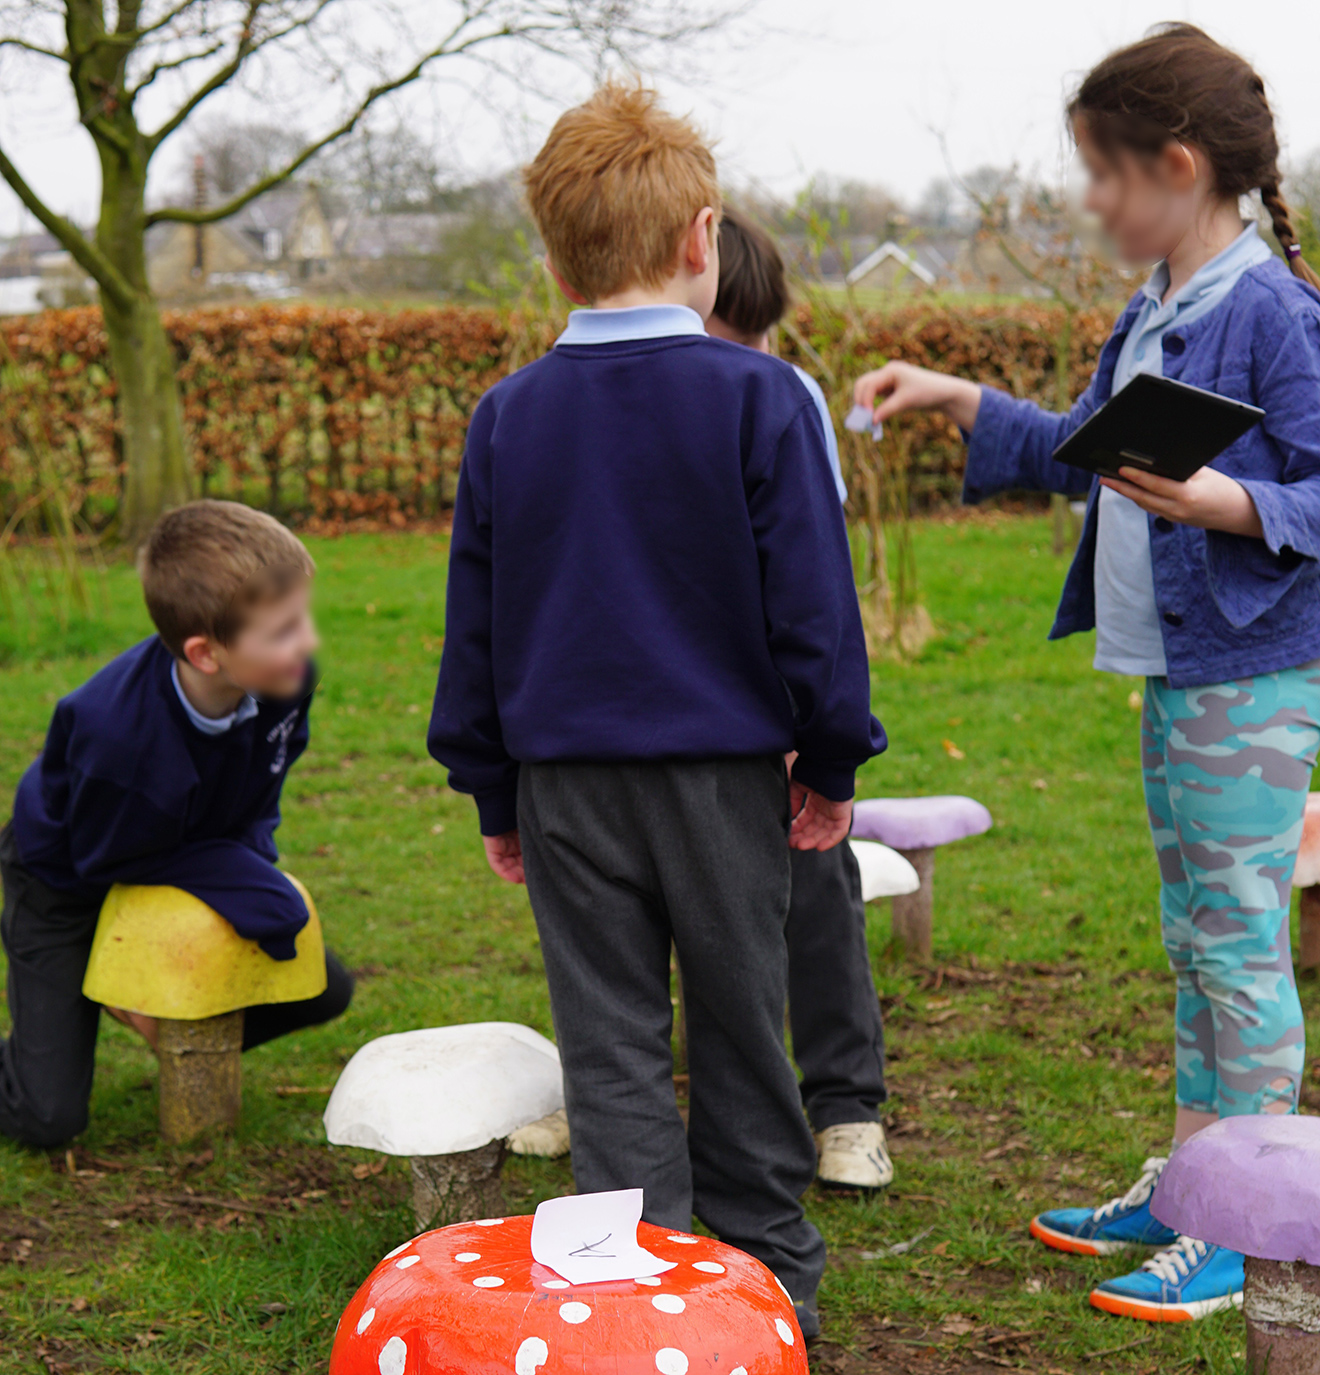
\includegraphics[width=0.8\columnwidth]{figures/mushrooms}
  \caption{A Year 4 student reveals a clue to her Activity's next puzzle. }~\label{fig:Mushrooms}
\end{figure}

\subsection{Study 3: Without Introducing the Medium (-RPA-E)}

\subsection{Planning the Full Curriculum (IRPAPE)}

\section{Discussion}

\subsection{Students' Desire for Independence}

\subsection{Focusing on Medium over Domain}

\subsection{Mobile Learning Activities as the Object}
Requires activity theory?

\subsection{Local Heritage as a Learning Resource}

\section{Conclusion}

\section{Acknowledgments}

% BALANCE COLUMNS
\balance{}

% REFERENCES FORMAT
% References must be the same font size as other body text.
\bibliographystyle{SIGCHI-Reference-Format}
\bibliography{sample}

\end{document}

%%% Local Variables:
%%% mode: latex
%%% TeX-master: t
%%% End:
